% !TeX spellcheck = en_US
% !TeX encoding = UTF-8
\section{Umbrella Sampling\label{Sec:ES:US}}
Umbrella Sampling method was proposed by Torrie and Valleau in 1977,\cite{TorrieJComputP1977} and is still widely used nowadays.
Suppose we are studying a transition process between states such as conversion between two dominant conformations or a chemical reaction, and these two states are separated by a high barrier relative to $kT$. Therefore, the transition is a rare event. A schematic representation of the free energy landscape is shown in Fig.~\ref{Fig:ES:dual_harmonic}.
\begin{figure}[htbp]
	\centering
%	\resizebox{2cm}{!}{
		\begin{tikzpicture}
		\def\lims{xmin=-5,xmax=5,ymin=-30,ymax=14}
		\begin{axis}[\lims,hide x axis, hide y axis,width=0.65\textwidth,height=0.4\textwidth]
           \addplot[mark=none,smooth,domain=-5:5] {0.4*((x+2)*(x-2))*((x+2)*(x-2))-4*x*x};
		\end{axis}
		\end{tikzpicture}
%	}
	\caption{A typical free energy surface. Two free energy wells are separated by a barrier higher than $kT$.}\label{Fig:ES:dual_harmonic}
\end{figure}

%\begin{figure}[htbp]
%	\centering
%	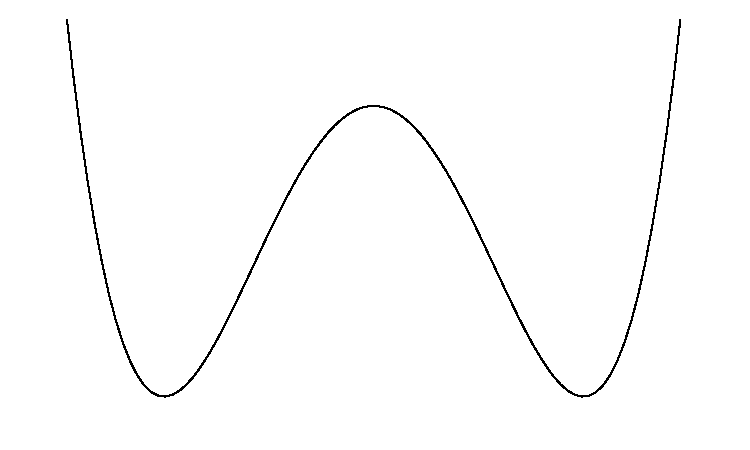
\includegraphics[width=0.6\textwidth]{figures/dual_harmonic.pdf}\\
%	\caption{A typical free energy surface. Two free energy barriers are separated by a barrier higher than $kT$.}\label{Fig:ES:dual_harmonic}
%\end{figure}

Sometimes, we are interested in not only these two dominate states but also the states in between. Usually, we define a reaction coordinate $\xi$ and calculate the potential of mean force along this reaction coordinate from the ``reactant'' to the ``product''. The reaction coordinate can be either real coordinates such as the difference of bond lengths in, for example, an $S_N2$ reaction, or it can be a thermodynamics coupling parameter ($\lambda$) that defines an unphysical path. However, if we run a simulation with the reaction coordinate initially set to the transition state or the slope, the system will quickly roll back to the ``reactant'' or the ``product'' state in order to reduce the free energy. The consequence is that phase space outside the ``reactant'' and ``product'' regions cannot be sampled sufficiently to yield accurate free energy profile in a brutal force simulation. In order to enhance the exploration in these regions, 
a series of artificial biasing potentials as (usually harmonic) functions of $\xi$ can be added to the potential energy. And the simulations are performed on these potential energy surfaces 
\begin{equation}
	U_i(\mathbf{R})=U_0(\mathbf{R})+\Delta U_i(\xi).
\end{equation}
Each biased simulation is called a \textit{window}. The strengths of the biases should be strong enough to maintain the system in the vicinity of where you are interested in, and also should be weak enough that the system can have significant overlap in two adjacent windows. After all the simulations, the whole region is well sampled. Ensemble average under $U_0$ can be calculated from the ensembles generated under the biased Hamiltonians $U$ via
\begin{align}
	\left<X(\mathbf{R})\right>_0=&\frac{\int X(\mathbf{R})\exp{\left[-\beta U_0(\mathbf{R})\right]}\diff\mathbf{R}}{\int \exp{\left[-\beta U_0(\mathbf{R})\right]}\diff\mathbf{R}}\notag\\
	                            =&\frac{\int X(\mathbf{R})\exp{\left[\beta \Delta U_i(\mathbf{R})\right]}\exp{\left[-\beta U_i(\mathbf{R})\right]}\diff\mathbf{R}}{\int \exp{\left[\beta \Delta U_i(\mathbf{R})\right]}\exp{\left[-\beta U_i(\mathbf{R})\right]}\diff\mathbf{R}}\notag\\
	                =&\frac{\left<X\exp{\left(\beta\Delta U_i\right)}\right>_i}{\left<\exp{\left(\beta\Delta U_i\right)}\right>_i}.
\end{align}
Better postprocessing methods are the Weighted Histogram Analysis Method and the Multistate Bennett Acceptance Ratio method (to be discussed in Section~\ref{Sec:FEM:WHAM} and~\ref{Sec:FEM:MBAR}).